% Created 2025-05-08 qui 15:52
% Intended LaTeX compiler: xelatex
\documentclass[a4paper,12pt]{article}
\usepackage{graphicx}
\usepackage{longtable}
\usepackage{wrapfig}
\usepackage{rotating}
\usepackage[normalem]{ulem}
\usepackage{capt-of}
\usepackage{hyperref}
\usepackage[brazil, ]{babel}
\usepackage{fontspec}
\setmainfont{Latin Modern Sans}
\usepackage{geometry}
\geometry{top=2.5cm,bottom=2.5cm,left=2.5cm,right=2.5cm}
\author{Gustavo de Tarso}
\date{\today}
\title{Sistemas de Saúde no Brasil – Resumo Completo}
\hypersetup{
 pdfauthor={Gustavo de Tarso},
 pdftitle={Sistemas de Saúde no Brasil – Resumo Completo},
 pdfkeywords={},
 pdfsubject={},
 pdfcreator={Emacs 30.0.91 (Org mode 9.7.11)}, 
 pdflang={Pt_Br}}
\begin{document}

\maketitle
\section{Parte 1/5 – Histórico, Desenvolvimento e Modelos de Análise dos Sistemas de Saúde no Brasil}
\label{sec:orgd265d90}

\subsection{Conceito de Sistema de Saúde}
\label{sec:orgad75a1d}
Um sistema de saúde é um conjunto de organizações, indivíduos, ações e relações institucionais, políticas e econômicas que interagem com o objetivo de promover, restaurar e manter a saúde de uma população. Envolve tanto atores públicos quanto privados e filantrópicos, regulados por normas e políticas governamentais, especialmente pelo Ministério da Saúde. Atua em níveis variados, da promoção à reabilitação, abrangendo programas como o PNI, vigilâncias sanitária e epidemiológica, saneamento básico, entre outros.
\subsection{Desenvolvimento Histórico do Sistema de Saúde no Brasil}
\label{sec:org3aa361e}

\subsubsection{Brasil Colônia (1500-1816)}
\label{sec:org64f67d3}
\begin{itemize}
\item Ausência de uma política pública estruturada.
\item Saúde limitada às Santas Casas de Misericórdia (SCM), fundadas por doações da comunidade.
\item Atendimento centrado em urgências e internações precárias.
\item Presença apenas de profissionais estrangeiros.
\end{itemize}
\subsubsection{Brasil Império (1816-1889)}
\label{sec:org90cda5d}
\begin{itemize}
\item Criação das primeiras escolas médicas em 1808 (RJ e BA).
\item Ênfase nas epidemias e sanitização portuária.
\item D. Pedro II impulsionou a institucionalização com Faculdades Médicas.
\item Revolta da Vacina (1904) marca o início da tensão entre Estado e população em políticas sanitárias.
\end{itemize}
\subsubsection{República Velha e Era Vargas (1889–1960)}
\label{sec:orgfaa8e35}
\begin{itemize}
\item Criação das CAPs (Caixas de Aposentadoria e Pensões) em 1923, financiadas por trabalhadores e empregadores.
\item Unificação em IAPs nos anos 1940.
\item Fundação do Ministério da Saúde em 1953.
\item INPS (1966) e posteriormente INAMPS (1977) centralizaram a previdência e assistência médica.
\end{itemize}
\subsubsection{Ditadura Militar (1964–1985)}
\label{sec:org7587a30}
\begin{itemize}
\item Sistema excludente: apenas trabalhadores com carteira assinada tinham acesso à saúde via INAMPS.
\item Forte concentração dos recursos no Sudeste.
\item Crescimento de desigualdades regionais.
\end{itemize}
\subsubsection{Constituição de 1988 e Criação do SUS}
\label{sec:org442e7a9}
\begin{itemize}
\item Estabeleceu a saúde como um direito universal.
\item Lei Orgânica da Saúde (Lei 8.080/1990) estruturou o SUS.
\item Diretrizes fundamentais: universalidade, equidade, integralidade, descentralização, participação popular e resolubilidade.
\item EC 29 (2000) fixou mínimos obrigatórios de investimento para estados (12\%) e municípios (15\%).
\item Criação da ANVISA em 1999 como órgão regulador sanitário.
\end{itemize}
\subsection{Atenção Primária à Saúde (APS)}
\label{sec:orgb1f7dae}
A APS é a principal porta de entrada do SUS e deve resolver até 85\% dos casos. Estruturada com base na longitudinalidade, integralidade, coordenação do cuidado e centralidade na comunidade. As UBSs são os principais dispositivos desse nível. No Brasil, políticas como a Estratégia Saúde da Família (1994) e a PNAB (2006) fortaleceram esse modelo.
\subsection{Problemas Estruturais do SUS}
\label{sec:orgb8a1b13}
\begin{itemize}
\item Subfinanciamento crônico.
\item Má gestão.
\item Escassez de profissionais especializados.
\item Longo tempo de espera para atendimento especializado.
\item Falta de leitos para procedimentos hospitalares.
\end{itemize}
\subsection{Índice de Desempenho do SUS (IDSUS)}
\label{sec:org50cbdff}
Criado em 2012, avaliava o SUS com base em acesso e efetividade. Apesar de ter sido descontinuado, revelou desigualdades regionais: Norte e Nordeste com os piores índices, Sul e Sudeste com os melhores. A nota média foi 5,47 em escala de 0 a 10.
\subsection{Sistema Privado de Saúde}
\label{sec:org5d2b5ee}
A saúde suplementar teve origem nas CAPs (1923) e ganhou força com as cooperativas e medicinas de grupo. Hoje, inclui diversas modalidades: seguradoras, autogestões, cooperativas médicas, filantrópicas e medicinas de grupo. Regulada pela ANS (Lei 9.656/98 e Lei 9.961/00).
\subsection{Questões sugeridas (FGV – discursivas)}
\label{sec:orgd5ea299}

\subsubsection{Questão 1}
\label{sec:orgabfae11}
Explique o processo histórico que levou à criação do Sistema Único de Saúde (SUS) e destaque seus principais pilares.

Resposta:
O SUS surgiu no contexto da redemocratização do Brasil, consolidando-se na Constituição de 1988. Antes disso, o modelo previdenciário limitava o acesso à saúde apenas aos trabalhadores formais, excluindo boa parte da população. A 8ª Conferência Nacional de Saúde (1986) foi um marco ao estabelecer a saúde como direito universal. O SUS foi estruturado pela Lei 8.080/90 com os seguintes pilares: universalidade, integralidade, equidade, descentralização, regionalização, participação popular e resolubilidade.
\subsubsection{Questão 2}
\label{sec:org99d5aef}
Compare o sistema de saúde brasileiro antes e depois da Constituição de 1988, considerando aspectos de acesso, financiamento e organização.

Resposta:
Antes de 1988, o acesso à saúde era limitado a trabalhadores com carteira assinada, gerando desigualdade e exclusão. O sistema era fragmentado, com forte centralização e financiamento limitado. Após a Constituição, o SUS promoveu acesso universal e igualitário, descentralizou a gestão e criou fontes de financiamento tripartite. Entretanto, desafios como subfinanciamento e desigualdades regionais persistem.
\section{Parte 2/5 – Modelos Internacionais e Comparativos de Sistemas de Saúde}
\label{sec:org9662140}

\subsection{Introdução aos Modelos de Sistemas de Saúde}
\label{sec:org78288c1}
Os sistemas de saúde pelo mundo se organizam conforme diferentes estruturas de financiamento, prestação de serviço, regulação e cobertura populacional. Para analisá-los comparativamente, utilizam-se categorias como: acesso universal, cobertura pública x privada, papel do Estado, e modelo de remuneração.

Segundo a OMS, os sistemas devem buscar três objetivos principais: (1) melhorar a saúde da população; (2) responder às expectativas das pessoas; (3) garantir proteção financeira contra os custos da doença.
\subsection{Modelo de Beveridge (Inglaterra)}
\label{sec:orgdfeffeb}
Criado no Reino Unido com o NHS (National Health Service) após a Segunda Guerra Mundial, o modelo Beveridgiano é financiado via impostos gerais. O Estado é o provedor principal dos serviços, que são públicos e gratuitos no ponto de atendimento. Caracteriza-se por:

\begin{itemize}
\item Universalidade de cobertura.
\item Financiamento público por impostos.
\item Hospitais públicos e médicos assalariados.
\item Foco em controle de custos e acesso.
\end{itemize}

Exemplo: Reino Unido, Espanha, Itália, Cuba, países escandinavos.
\subsection{Modelo de Bismarck (Alemanha)}
\label{sec:orgc2e41f0}
Fundado na Alemanha por Otto von Bismarck no século XIX, é baseado em um seguro social obrigatório. As contribuições vêm de empregadores e empregados. Os prestadores são privados, mas regulados.

\begin{itemize}
\item Caráter contributivo (folha de pagamento).
\item Várias "caixas de seguro saúde" (sickness funds).
\item Prestadores privados ou públicos.
\item Cobertura ampla, mas dependente de vínculo empregatício.
\end{itemize}

Exemplo: Alemanha, França, Japão, Bélgica, Suíça.
\subsection{Modelo de Mercado (Estados Unidos)}
\label{sec:orgd128977}
Baseado na lógica de mercado, com papel limitado do Estado. A cobertura é garantida por seguros privados, em sua maioria, contratados individualmente ou via empregador.

\begin{itemize}
\item Forte presença do setor privado.
\item Planos variados e fragmentados.
\item Cobertura parcial via Medicaid (população vulnerável) e Medicare (idosos).
\item Alto custo e desigualdade no acesso.
\end{itemize}
\subsection{Sistema Canadense (Modelo Nacional de Saúde com Gestão Descentralizada)}
\label{sec:org5065bcf}
O Canadá possui um sistema público universal com gestão descentralizada pelas províncias. Os médicos são privados, mas pagos pelo governo por serviço prestado (fee-for-service).

\begin{itemize}
\item Universalidade com financiamento público.
\item Sistema de pagador único (single-payer system).
\item Proibição da duplicação de serviços privados cobertos publicamente.
\item Baixos custos administrativos.
\end{itemize}
\subsection{Sistema de Saúde Brasileiro: Comparações e Contradições}
\label{sec:org5b6c922}
O SUS é uma referência mundial pela sua universalidade. No entanto, sofre com subfinanciamento crônico, judicialização excessiva e sobreposição com o setor suplementar. Em contraste, países com modelos semelhantes ao Beveridge, como o Reino Unido, mantêm maior controle sobre custos e planejamento assistencial.
\subsection{Principais Indicadores Comparativos}
\label{sec:orgc8c1239}
\begin{itemize}
\item Gasto em saúde (\% do PIB): Brasil (9,2\%), Reino Unido (10,2\%), Alemanha (11,7\%), EUA (16,9\%).
\item Expectativa de vida: Brasil (76 anos), Alemanha (81), Japão (84), EUA (77).
\item Mortalidade infantil: Brasil (12/1000), Alemanha (3), EUA (5,4).
\item Cobertura populacional: Brasil (SUS cobre 75\%), Reino Unido (100\%), EUA (±90\%, após ACA).
\end{itemize}
\subsection{Questões sugeridas (FGV – discursivas)}
\label{sec:orgf073cbd}

\subsubsection{Questão 1}
\label{sec:org873941f}
Compare os modelos de Beveridge, Bismarck e o Sistema de Saúde Brasileiro, considerando financiamento, acesso e regulação.

Resposta:
O modelo de Beveridge é financiado via impostos e provido pelo Estado, com acesso universal e forte regulação pública. O modelo Bismarck é baseado em seguros sociais, com gestão mais descentralizada e maior presença do setor privado. O Brasil possui um sistema de inspiração Beveridgiana (SUS), com acesso universal gratuito, porém convive com um setor privado robusto e fragmentação na gestão. O financiamento no Brasil é subdimensionado em comparação com países da OCDE, o que compromete a equidade e eficiência.
\subsubsection{Questão 2}
\label{sec:org24b0f38}
Explique as principais vantagens e limitações dos modelos de saúde baseados no mercado, tomando os Estados Unidos como referência.

Resposta:
O modelo de mercado permite maior liberdade de escolha e inovação por parte dos prestadores. No entanto, apresenta alto custo, cobertura desigual e barreiras de acesso. Nos Estados Unidos, a ausência de um sistema público universal resulta em milhões de pessoas sem seguro, alto endividamento por despesas médicas e iniquidades graves em saúde. A fragmentação e a falta de coordenação agravam a ineficiência sistêmica.
\section{Parte 3/5 – Estrutura e Organização dos Sistemas de Saúde no Brasil}
\label{sec:orgf48740d}

\subsection{Transição Demográfica e Epidemiológica}
\label{sec:orgbdbc459}
O Brasil vivencia uma transição demográfica acentuada, com redução da natalidade, queda da mortalidade e envelhecimento populacional. Paralelamente, ocorre a transição epidemiológica, com redução das doenças infectocontagiosas e aumento das doenças crônicas não transmissíveis (DCNT), como diabetes, hipertensão e câncer.

Essas mudanças pressionam o sistema de saúde, que precisa lidar com uma população mais idosa e dependente de cuidados prolongados e complexos.
\subsection{Determinantes Sociais de Saúde (DSS)}
\label{sec:org1954b62}
Conceito estabelecido pela OMS, os DSS são fatores econômicos, sociais, culturais e ambientais que afetam a saúde da população. Incluem:
\begin{itemize}
\item Educação, emprego, renda.
\item Moradia, saneamento, transporte.
\item Racismo, exclusão social, insegurança alimentar.
\item Acesso a serviços de saúde e alimentação saudável.
\end{itemize}

A abordagem baseada nos DSS exige ações intersetoriais e políticas públicas integradas.
\subsection{Envelhecimento da População}
\label{sec:orge32ab2e}
A pirâmide etária brasileira está se invertendo. Projeções indicam um aumento expressivo da população acima de 60 anos, com impacto direto nas aposentadorias e na demanda por serviços de saúde de alta complexidade.

Esse fenômeno demanda maior investimento em atenção primária, prevenção de agravos e reorganização da rede de cuidados de longa duração.
\subsection{Estratégia Saúde da Família (ESF)}
\label{sec:orga5a7964}
A ESF reorganiza a Atenção Primária à Saúde (APS) no Brasil. É composta por equipes multidisciplinares (médico, enfermeiro, técnico, agente comunitário de saúde) que atuam em áreas geográficas definidas, com enfoque na promoção da saúde, prevenção de doenças, e vigilância em saúde.

A ESF é um dos pilares do SUS e tem contribuído para a melhoria dos indicadores de saúde, como redução da mortalidade infantil e aumento da cobertura vacinal.
\subsection{Itens Preocupantes na Gestão do SUS}
\label{sec:org716cabe}
\begin{itemize}
\item Aumento das condições crônicas.
\item Judicialização da saúde.
\item Baixa transparência na relação público-privado.
\item Fragmentação da gestão e baixa resolubilidade.
\item Subfinanciamento persistente.
\end{itemize}
\subsection{Financiamento do SUS}
\label{sec:orgfe3ea22}
O financiamento é público e dividido entre União, Estados e Municípios (sistema tripartite). Os principais blocos de custeio incluem:
\begin{itemize}
\item Atenção básica.
\item Média e alta complexidade.
\item Vigilância em saúde.
\item Assistência farmacêutica.
\end{itemize}

A tabela de procedimentos (SIGTAP) define os valores pagos aos serviços prestados. O subfinanciamento e o congelamento de gastos (EC 95/2016) impactam diretamente a capacidade do sistema.
\subsection{Governança do SUS}
\label{sec:orgef0031d}
O SUS é coordenado pelo Ministério da Saúde e descentralizado entre estados e municípios. As principais instâncias de pactuação são:
\begin{itemize}
\item CIT (Comissão Intergestores Tripartite).
\item CIB (Comissão Intergestores Bipartite).
\item Conselhos de saúde (níveis federal, estadual e municipal).
\end{itemize}

O modelo participativo é fundamental, com destaque para o controle social exercido por usuários, profissionais e gestores.
\subsection{Protocolos Clínicos e Diretrizes Terapêuticas (PCDT)}
\label{sec:orgd33a306}
Instrumentos que definem critérios para diagnóstico, tratamento, posologia e monitoramento de agravos à saúde. São fundamentais para garantir equidade, racionalidade do uso de recursos e segurança clínica.
\subsection{Telesaúde e Conecte SUS}
\label{sec:org801e7f6}
Programas que visam melhorar o acesso e qualidade da atenção, com uso de tecnologia para orientação de condutas, teleconsultas, segunda opinião e interoperabilidade de dados.
\subsection{Oportunidades de Melhoria}
\label{sec:orgd57e19e}
\begin{itemize}
\item Integração das redes de atenção à saúde.
\item Expansão do uso de prontuário eletrônico.
\item Melhoria da jornada do paciente.
\item Educação permanente dos profissionais.
\item Aprimoramento da regulação (vaga zero, por exemplo).
\end{itemize}
\subsection{Questões sugeridas (FGV – discursivas)}
\label{sec:orgf30286a}

\subsubsection{Questão 1}
\label{sec:org7a5533c}
Analise os impactos da transição demográfica e epidemiológica sobre o SUS, destacando os desafios e estratégias para enfrentá-los.

Resposta:
A transição demográfica, com o envelhecimento populacional, e a epidemiológica, com o aumento das doenças crônicas, impõem novos desafios ao SUS. A demanda por cuidados contínuos, exames, medicamentos e internações cresce, pressionando os recursos do sistema. Estratégias incluem fortalecimento da Atenção Primária à Saúde, adoção de modelos de cuidado centrados no paciente, ampliação de equipes multiprofissionais e investimentos em prevenção e telessaúde. A ESF se mostra central neste processo.
\subsubsection{Questão 2}
\label{sec:org63649b0}
Explique a importância dos determinantes sociais da saúde na formulação de políticas públicas e como eles podem ser integrados ao planejamento do SUS.

Resposta:
Os DSS representam fatores como educação, renda, saneamento, alimentação e trabalho que influenciam diretamente os níveis de saúde. Políticas públicas que desconsideram esses determinantes tendem a ser ineficazes. Integrar os DSS ao SUS significa articular ações intersetoriais, por meio de políticas integradas com educação, habitação, transporte e assistência social. O planejamento territorial e o mapeamento de vulnerabilidades são ferramentas importantes nesse processo.
\section{Parte 4/5 – Poder do Paciente e Modelos de Remuneração em Saúde}
\label{sec:orgea4af87}

\subsection{Introdução aos Modelos de Remuneração}
\label{sec:org490d0cb}
A forma como os serviços de saúde são pagos influencia diretamente o comportamento dos prestadores, os custos do sistema e os desfechos clínicos. Os modelos de remuneração refletem diferentes estratégias para alinhar incentivos e resultados em saúde, variando entre:
\begin{itemize}
\item Fee-for-Service (FFS)
\item Capitation
\item Pagamento por desempenho (P4P)
\item Bundled payments
\item DRG (Diagnosis-Related Groups)
\item VBHC (Value-Based Health Care)
\end{itemize}
\subsection{Fee-for-Service (FFS)}
\label{sec:org4989ffe}
Modelo predominante no Brasil. Remunera-se por cada procedimento realizado, o que pode estimular o excesso de exames, consultas e internações. Incentiva volume, não necessariamente qualidade.
\subsection{Capitation}
\label{sec:org70b54fd}
Pagamento prospectivo e per capita. Um valor fixo mensal é pago para o atendimento de um grupo de pessoas, independentemente do número de procedimentos realizados. É comum em modelos de atenção primária, focando em prevenção e cuidado contínuo.
\subsection{Bundled Payments}
\label{sec:org2bfa266}
Pagamentos por episódio de cuidado. Engloba todos os serviços relacionados a um tratamento ou condição (ex: parto, cirurgia cardíaca). Busca previsibilidade e controle de custos, promovendo gestão integrada.
\subsection{DRG – Diagnosis-Related Groups}
\label{sec:org4c743b9}
Sistema baseado em grupos de diagnósticos clínicos semelhantes. O pagamento cobre todo o cuidado relacionado ao diagnóstico, ajustado por complexidade e comorbidades. Usado em países como EUA e Alemanha.
\subsection{Pagamento por Desempenho (Pay-for-Performance - P4P)}
\label{sec:org6485a03}
Bonificações ou penalizações são aplicadas com base em indicadores de qualidade, segurança e desfechos clínicos. Promove eficiência e resultados mensuráveis.
\subsection{VBHC – Value-Based Health Care}
\label{sec:org1489c64}
Baseado em valor para o paciente. Relaciona os custos aos desfechos clínicos e à experiência do cuidado. Exige sistemas de informação robustos e acompanhamento de indicadores como PREMS e PROMS.
\subsection{Valor em Saúde: PREMS e PROMS}
\label{sec:orga4a00d6}
\begin{itemize}
\item PREMS (Patient Reported Experience Measures): captam a experiência do paciente com o atendimento.
\item PROMS (Patient Reported Outcome Measures): medem os resultados relatados pelo próprio paciente.
\end{itemize}

Esses indicadores são centrais para o modelo de saúde baseado em valor.
\subsection{Auditoria em Saúde Suplementar}
\label{sec:org364f9b5}
Existem três tipos de auditoria:
\begin{itemize}
\item Prospectiva: análise prévia de solicitações.
\item Concorrente: durante a internação.
\item Retrospectiva: após a alta, focando em análise documental.
\end{itemize}
\subsection{Suficiência de Rede e Cobertura Assistencial}
\label{sec:org74b0f22}
A ANS estabelece critérios mínimos de cobertura para planos de saúde, bem como prazos para atendimento, que incluem:
\begin{itemize}
\item 7 dias para consulta básica.
\item 14 dias para especialidades.
\item 3 dias para exames simples.
\end{itemize}

A NIP (Notificação de Intermediação Preliminar) é o principal mecanismo de mediação de conflitos entre usuários e operadoras.
\subsection{Empoderamento do Paciente (Empowerment)}
\label{sec:org9270623}
Refere-se à capacidade do paciente de tomar decisões informadas sobre seu cuidado. É fomentado por:
\begin{itemize}
\item Acesso à informação (Health 2.0).
\item Autocuidado em doenças crônicas.
\item Participação ativa em decisões clínicas.
\end{itemize}

O movimento Health 2.0 integra aplicativos, prontuário eletrônico e dados pessoais com dispositivos vestíveis (wearables) e plataformas digitais, promovendo protagonismo do paciente.
\subsection{Questões sugeridas (FGV – discursivas)}
\label{sec:org45131e1}

\subsubsection{Questão 1}
\label{sec:org01c5b55}
Explique as principais vantagens e riscos do modelo de remuneração Fee-for-Service (FFS) e apresente alternativas mais eficientes.

Resposta:
O modelo FFS remunera prestadores por procedimentos realizados, incentivando o volume de atendimentos, o que pode resultar em excesso de exames e terapias desnecessárias, aumento de custos e riscos ao paciente. Apesar de sua simplicidade e previsibilidade, não estimula a coordenação do cuidado nem a melhoria dos desfechos. Alternativas mais eficientes incluem o capitation, que remunera com foco em prevenção e gestão da população, e modelos baseados em valor (VBHC), que alinham pagamento a resultados clínicos.
\subsubsection{Questão 2}
\label{sec:orge67f627}
Discorra sobre o papel do empoderamento do paciente nos novos modelos de atenção à saúde e como ele pode contribuir para a eficiência dos sistemas de saúde.

Resposta:
O empoderamento do paciente permite maior participação nas decisões de tratamento, adesão terapêutica e autocuidado, especialmente em condições crônicas. Isso resulta em melhor controle de doenças, menor utilização de serviços de emergência e melhora nos desfechos clínicos. A digitalização da saúde (prontuário eletrônico, apps, telessaúde) facilita esse protagonismo, permitindo decisões mais informadas. Em modelos como o VBHC, a experiência e os resultados relatados pelo paciente são parte central da avaliação dos serviços prestados.
\section{Parte 5/5 – Tendências e Reflexões sobre os Sistemas de Saúde}
\label{sec:orged8e2ad}

\subsection{Parcerias Público-Privadas (PPP)}
\label{sec:orgf0076cf}
As PPPs são instrumentos que visam unir recursos do setor público e a expertise do setor privado para execução de serviços públicos. No setor saúde, podem assumir dois modelos:
\begin{itemize}
\item Administrativa: o Estado remunera o parceiro privado.
\item Patrocinada: há remuneração por tarifas cobradas dos usuários e complemento do Estado.
\end{itemize}

Embora não representem privatização, há risco de perda de controle público e conflitos de interesse. Sua execução requer cláusulas rígidas de avaliação de desempenho, metas, e penalidades.
\subsection{Terceiro Setor: OSS e OSCIP}
\label{sec:org9aa4878}
\begin{itemize}
\item \textbf{\textbf{OSS (Organizações Sociais de Saúde)}}: Entidades privadas sem fins lucrativos qualificadas pelo poder público. Podem gerir hospitais, UBS e outros equipamentos. Exigem conselhos com representação do Estado e da sociedade civil.
\item \textbf{\textbf{OSCIP (Organizações da Sociedade Civil de Interesse Público)}}: Têm funções mais amplas (educação, meio ambiente, saúde). Não gerem diretamente serviços públicos, mas realizam projetos via termos de parceria.
\end{itemize}

Ambas são formas de publicização e descentralização da gestão pública, frequentemente usadas para ampliar a capilaridade do SUS, embora existam críticas quanto à accountability e transparência.
\subsection{Fundações e Autarquias}
\label{sec:org3fe4242}
\begin{itemize}
\item \textbf{\textbf{Autarquias}} (ex: ANS, ANVISA, IBGE) são órgãos da administração indireta, com autonomia administrativa e financeira.
\item \textbf{\textbf{Fundações públicas e privadas}} são criadas para fins específicos (educação, pesquisa, saúde), com patrimônio próprio e autonomia.
\end{itemize}

Ambas têm papel relevante na regulação e execução das políticas públicas de saúde.
\subsection{Agenda 2030 e Metas para o Brasil}
\label{sec:org48dfd19}
Inspirada nos Objetivos de Desenvolvimento Sustentável (ODS), a Agenda 2030 para o Brasil estabelece:
\begin{enumerate}
\item Maior expectativa de vida da América Latina.
\item Menor mortalidade infantil.
\item Redução das desigualdades regionais em saúde.
\end{enumerate}

Essas metas demandam investimento em atenção primária, digitalização dos serviços e redução das iniquidades sociais.
\subsection{Caso de Sucesso: Estônia}
\label{sec:org0fd8a3b}
A Estônia é referência em digitalização estatal. Com a identificação eletrônica (e-ID), todos os serviços públicos são acessíveis digitalmente, inclusive os de saúde:
\begin{itemize}
\item Prontuário eletrônico acessível.
\item Prescrição digital integrada.
\item Ambulâncias via aplicativo.
\item Consultas por telemedicina.
\item Cidadãos têm acesso a todo o histórico médico e controle sobre quem acessa seus dados.
\end{itemize}

O sistema baseado em blockchain (X-Road) garante segurança, interoperabilidade e transparência, gerando economia de até 2\% do PIB.
\subsection{Transformação Digital na Saúde}
\label{sec:org627d1e3}
A digitalização é uma tendência irreversível no setor:
\begin{itemize}
\item Prontuário eletrônico e interoperabilidade.
\item Big data, analytics e inteligência artificial.
\item Telemedicina e dispositivos wearables.
\item Blockchain para segurança de dados.
\end{itemize}

Essas tecnologias, quando integradas, promovem maior eficiência, gestão baseada em evidência e empoderamento do cidadão.
\subsection{Desafios estruturais do SUS}
\label{sec:orgf045fd9}
\begin{itemize}
\item Falta de planejamento e continuidade administrativa.
\item Subfinanciamento e congelamento de gastos (EC 95).
\item Fragmentação da gestão e ausência de dados integrados.
\item Cultura institucional resistente à inovação.
\item Judicialização e baixa educação em saúde da população.
\end{itemize}
\subsection{Medidas de contenção e oportunidades}
\label{sec:orgf6d1414}
\begin{itemize}
\item Reformas no modelo de remuneração (VBHC, DRG).
\item Investimentos em APS, prevenção e promoção da saúde.
\item Educação digital da população.
\item Parcerias com o setor privado com accountability.
\item Melhoria na jornada do cidadão (regulação, encaminhamento, resolutividade).
\end{itemize}
\subsection{Questões sugeridas (FGV – discursivas)}
\label{sec:orgfa18a20}

\subsubsection{Questão 1}
\label{sec:org2264fc9}
Analise os benefícios e riscos do uso das Parcerias Público-Privadas (PPP) no sistema de saúde brasileiro. Como equilibrar eficiência e controle social?

Resposta:
As PPPs ampliam a capacidade de execução do Estado, permitem acesso a tecnologia e melhores práticas do setor privado, e podem acelerar entregas. No entanto, riscos como perda de controle público, corrupção e serviços com foco mercantilista existem. O equilíbrio exige contratos bem estruturados, metas claras, fiscalização rigorosa, e participação efetiva da sociedade civil por meio de conselhos e audiências públicas.
\subsubsection{Questão 2}
\label{sec:org6d6b71a}
Explique como a digitalização dos serviços públicos de saúde pode contribuir para o alcance das metas da Agenda 2030. Use o exemplo da Estônia como referência.

Resposta:
A digitalização permite monitoramento em tempo real dos indicadores de saúde, otimiza o acesso ao cuidado e reduz desperdícios. O exemplo da Estônia mostra que, com um sistema integrado de dados, é possível prever riscos, personalizar tratamentos e dar mais autonomia ao cidadão. No Brasil, isso pode melhorar o desempenho do SUS, especialmente em áreas remotas, e contribuir para metas como a redução da mortalidade infantil, aumento da expectativa de vida e combate às desigualdades regionais.
\section{Mapa Mental – Sistemas de Saúde no Brasil}
\label{sec:org968212f}

\begin{center}
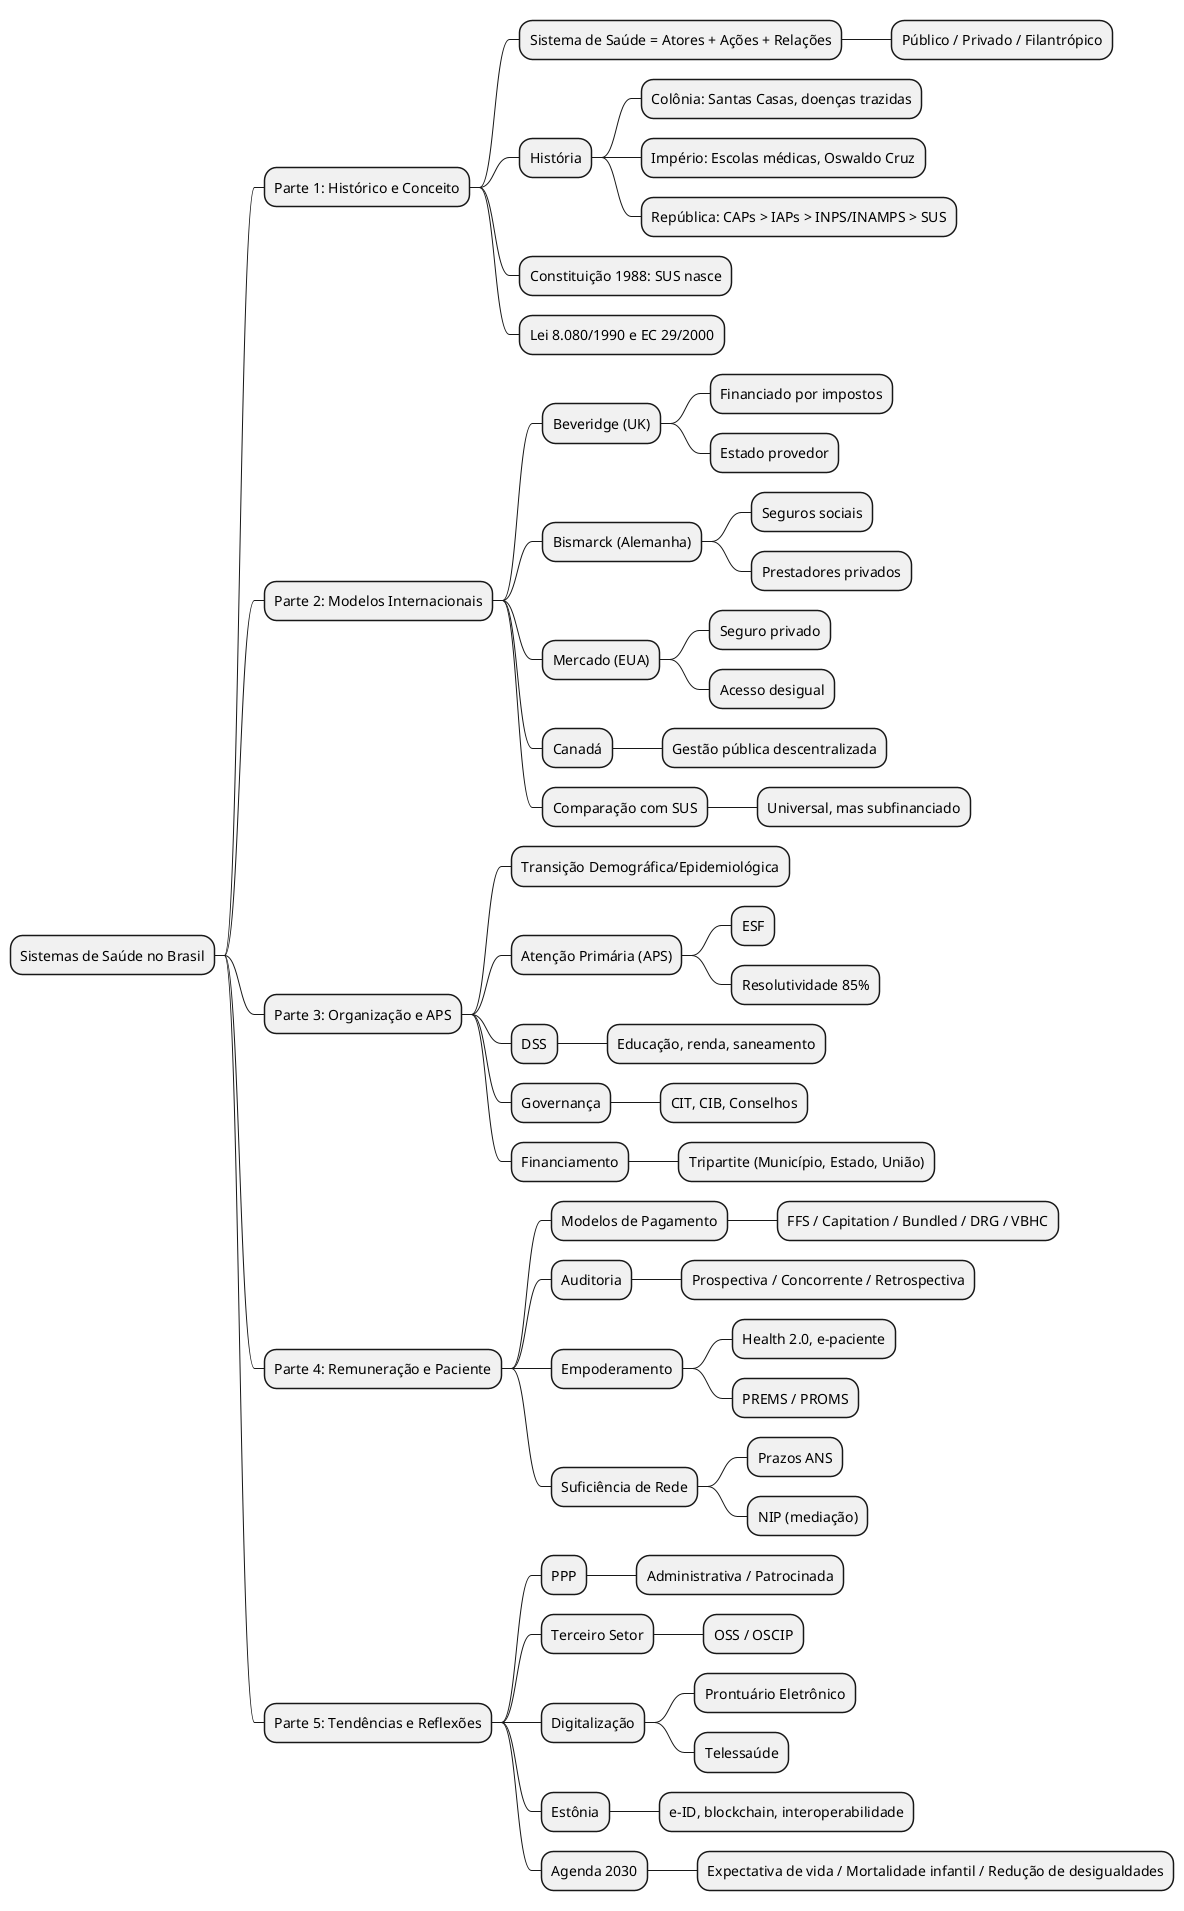
\includegraphics[width=.9\linewidth]{sistemas-saude-mapa.png}
\label{org1d1c1ce}
\end{center}
\end{document}
